\chapter{Cadre général du projet}

\section{Introduction}
Dans ce chapitre, nous commençons par la présentation de l'organisme d'accueil. Puis, nous mettons le projet dans son contexte général, en identifiant la problématique et en fixant ses objectifs. Finalement, nous présentons la méthodologie de travail adoptée dans ce projet.

\section{Présentation de l'organisme d'accueil}

NextStep IT \cite{NextStepIT} est un intégrateur spécialisé dans les métiers de l'infrastructure et dans les services liés aux nouvelles technologies, avec une offre complète qui va du conseil jusqu'à l'exploitation. Fondée en 2012, NextStep IT a rapidement évolué pour devenir un acteur clé dans le domaine des solutions cloud et des services IT. L'entreprise, basée à Charguia, s'est distinguée par son engagement à fournir des solutions innovantes et adaptées aux besoins de ses clients.

La mission de NextStep IT est de faciliter la transformation numérique des entreprises en leur offrant des solutions technologiques avancées, fiables et personnalisées. La vision de l'entreprise est de devenir le partenaire incontournable des entreprises souhaitant optimiser leur infrastructure IT et leurs processus métiers.

\begin{figure}[htpb]
\centering

\includegraphics[width=0.30\columnwidth]{image/nexsteplogo.png}
\caption{Logo de l'entreprise}
\label{fig:logo_nextstep}
\end{figure}

\subsection{Fiche d'identité de NextStep IT}

Le tableau~\ref{tab:coordonnees} présente la fiche d'identité de NextStep IT.

\begin{table}[h!]
\centering
\begin{tabular}{|l|l|}
\hline
Nom de la société & NextStep IT \\
\hline
Année de création & 2012 \\
\hline
Secteur d'activité & Infrastructure IT, Cloud et nouvelles technologies \\
\hline
Siège social & Charguia, Tunisie \\
\hline
Domaines d'intervention & Fournisseur Internet, Intégration, Cloud, Services Managés, Support et Assistance, Conseil \\
\hline
Logo & 
\includegraphics[width=3cm]{image/nexsteplogo.png} \\
\hline
\end{tabular}
\caption{Fiche d'identité de NextStep IT}
\label{tab:coordonnees}
\end{table}

\subsection{L'organigramme}

NextStep IT est structurée autour d'une direction générale supervisant les différents pôles opérationnels de l'entreprise (Cloud \& Infrastructure, Intégration \& Réseaux, Support \& Services Managés, Commercial, Conseil), chacun étant piloté par un responsable de pôle. Le stage s'est déroulé au sein du pôle Cloud, sous l'encadrement d'un ingénieur responsable des solutions d'infrastructure as a service.

\subsection{Domaines d'activité de NextStep IT}

NextStep IT accompagne ses clients à travers une offre complète et structurée autour de six grands pôles de services :

\begin{itemize}
    \item Fournisseur Internet :\\
    - Accès Internet haut débit sécurisé.\\
    - Services Internet personnalisés selon les usages métiers.\\
    - Solutions SD-WAN (réseau étendu piloté par logiciel, optimisé pour la performance et la résilience).

    \item Intégration :\\
    - Réseaux d'entreprise (réseaux locaux, Wifi, interconnexions, optimisation WAN, Data Center, QoS, câblage et supervision).\\
    - Solutions de mobilité et cybersécurité (sécurité périmétrique, VPN, WAF, IPS, antivirus, authentification forte, SIEM, PAM).\\
    - Data Center virtualisé, téléphonie IP, visioconférence.

    \item Cloud :\\
    - Housing, Infrastructure as a Service (IaaS).\\
    - Backup as a Service, Disaster Recovery.\\
    - Solutions de collaboration en ligne.

    \item Services Managés :\\
    - Prise en charge de l'infrastructure (ressources matérielles, réseaux, télécoms, applications).\\
    - Sécurité proactive, outils collaboratifs, haute disponibilité.\\
    - Supervision centralisée via NOC/SOC.

    \item Support et Assistance :\\
    - Assistance technique et maintenance.\\
    - Support technique (diagnostic et résolution d'incidents).\\
    - Infogérance complète.

    \item Conseil :\\
    - Audit de l'existant.\\
    - Études fonctionnelles et techniques, assistance à maîtrise d'ouvrage (AMOA).\\
    - Accompagnement stratégique et technologique.
\end{itemize}

C'est dans le pôle Cloud, et plus particulièrement dans une démarche de renforcement de l'offre Infrastructure as a Service, que s'inscrit notre projet de fin d'études : la conception et la réalisation d'une plateforme PaaS serverless bâtie sur Kubernetes, destinée à permettre aux clients de déployer et d'exploiter leurs applications conteneurisées sans avoir à gérer directement la complexité de l'orchestration sous-jacente.

\section{Contexte de Projet}

Dans cette section, nous décrivons la problématique, puis nous examinons la solution proposée, avant de préciser la méthodologie de travail adoptée.

\subsection{Problématique}

Ce projet est réalisé dans le cadre du Projet de Fin d'Études (PFE) du cycle ingénieur, en partenariat avec NextStep IT. Il s'inscrit dans une logique d'évolution de l'offre Cloud de l'entreprise : alors que l'IaaS traditionnel met à disposition des clients des ressources virtualisées brutes (machines virtuelles, stockage, réseau), la tendance du marché est de proposer des couches d'abstraction supplémentaires permettant aux équipes de développement de se concentrer sur leurs applications plutôt que sur l'administration de l'infrastructure.

\vspace{0.3cm}

L'objectif du projet est de concevoir, développer et déployer une plateforme de type PaaS (Platform as a Service) serverless multi-tenant, reposant sur un cluster Kubernetes et exploitant les technologies Knative Serving et Knative Eventing pour offrir des capacités de mise à l'échelle automatique (y compris la mise à l'échelle à zéro instance), ainsi qu'un modèle de facturation à l'usage. La plateforme s'appuie également sur Apache Kafka, opéré via l'opérateur Strimzi, pour la prise en charge de charges de travail pilotées par événements (event-driven).

\vspace{0.3cm}

Le déploiement et l'exploitation d'applications conteneurisées sur Kubernetes exigent une expertise technique pointue : configuration des ressources, gestion des espaces de noms (namespaces), mise en place de l'autoscaling, gestion du cycle de vie des révisions, supervision de la charge, sécurisation des flux réseau entre locataires (tenants), etc. Cette complexité constitue un frein important pour des équipes de développement qui souhaitent déployer rapidement leurs applications sans pour autant investir dans la maîtrise complète de l'écosystème Kubernetes.

\vspace{0.3cm}

Par ailleurs, les modèles de facturation classiques de l'hébergement (instances réservées, facturation forfaitaire) sont peu adaptés à des charges de travail variables ou intermittentes, où une application peut rester inactive une grande partie du temps. Un modèle de facturation à l'usage, aligné sur la consommation réelle de ressources (CPU, mémoire, temps d'activité), répond mieux à ce type de besoin.

\vspace{0.5cm}

\noindent La problématique peut donc être résumée comme suit :

\vspace{0.3cm}

\begin{center}
\fbox{
\parbox{0.9\textwidth}{
\centering

Comment concevoir une plateforme PaaS serverless multi-tenant, bâtie sur Kubernetes, permettant aux clients de déployer et d'exploiter des applications conteneurisées de manière autonome et sécurisée, avec une mise à l'échelle automatique incluant le retour à zéro instance, une intégration native avec un système de messagerie événementielle, et une facturation reflétant l'usage réel des ressources ?

}
}
\end{center}

\subsection{Étude de l'existant}

Plusieurs solutions existent aujourd'hui sur le marché pour répondre, partiellement ou totalement, à cette problématique.

\subsubsection*{Heroku}
Pionnier du PaaS, Heroku propose une expérience de déploiement très simplifiée (git push pour déployer), mais reste une plateforme propriétaire et fermée, offrant peu de contrôle sur l'infrastructure sous-jacente et dont les coûts croissent rapidement à l'échelle.

\subsubsection*{AWS Lambda / Google Cloud Run / Azure Container Apps}
Solutions serverless managées par les principaux fournisseurs de cloud public. Elles offrent une excellente mise à l'échelle automatique, mais imposent un verrouillage fort vis-à-vis du fournisseur (vendor lock-in) et ne peuvent pas être hébergées sur une infrastructure privée ou on-premise, ce qui pose un problème pour un intégrateur comme NextStep IT souhaitant proposer une offre maîtrisée sur son propre cluster.

\subsubsection*{OpenShift (Red Hat)}
Plateforme PaaS complète bâtie sur Kubernetes, très robuste mais lourde à opérer et sous licence commerciale, avec un coût d'entrée élevé peu compatible avec une offre destinée à des PME.

\subsubsection*{Knative (projet open source, CNCF)}
Brique logicielle bâtie au-dessus de Kubernetes, apportant nativement les fonctionnalités de scale-to-zero et d'autoscaling par requêtes (Knative Serving), ainsi qu'un modèle événementiel standardisé (Knative Eventing). Contrairement aux solutions précédentes, Knative est open source, peut être déployé sur n'importe quel cluster Kubernetes (y compris on-premise), et ne fournit pas de portail utilisateur ni de couche de gestion multi-tenant, de facturation ou d'administration : il s'agit d'une brique d'infrastructure, pas d'une plateforme clé en main.

\subsubsection*{Conclusion de l'étude de l'existant}

Cette étude de l'existant met en évidence un vide entre, d'une part, les briques open source performantes mais non finies (Knative, Strimzi) et, d'autre part, les plateformes commerciales complètes mais fermées ou coûteuses (Heroku, OpenShift, offres serverless propriétaires des hyperscalers). C'est précisément cet espace que notre projet vise à occuper : construire, au-dessus de briques open source éprouvées, une plateforme PaaS serverless complète, multi-tenant, avec portail applicatif, facturation à l'usage et console d'administration, hébergeable sur l'infrastructure propre de l'intégrateur.

\subsection{Solution proposée}

La solution proposée consiste en une plateforme PaaS serverless multi-tenant articulée autour des composants suivants :

\begin{itemize}
    \item Un cluster Kubernetes comme socle d'orchestration, sur lequel chaque client (tenant) dispose de son propre espace de noms isolé par des règles réseau (NetworkPolicy).
    \item Knative Serving pour l'exécution des applications des clients sous forme de services capables de monter en charge automatiquement en fonction du trafic, et de redescendre jusqu'à zéro instance en l'absence de sollicitation, réduisant ainsi la consommation de ressources et le coût pour le client.
    \item Apache Kafka, opéré par l'opérateur Strimzi sur Kubernetes, comme bus d'événements permettant aux applications des clients de communiquer de manière asynchrone.
    \item Knative Eventing, qui relie les messages Kafka aux services Knative via les ressources Broker, Trigger et KafkaSource, permettant de réveiller automatiquement une application mise à zéro instance à la réception d'un événement.
    \item Un backend applicatif développé en Spring Boot, exposant une API REST sécurisée, orchestrant le cluster Kubernetes via le client Java Fabric8, et portant la logique métier (gestion des utilisateurs, des applications, de la facturation, des clés d'API, des journaux).
    \item Deux portails web développés en React : un portail client permettant aux locataires de déployer et de superviser leurs applications, et une console d'administration réservée à l'équipe exploitant la plateforme.
    \item Keycloak comme fournisseur d'identité, assurant l'authentification et la gestion des rôles (administrateur de la plateforme, administrateur de compte client, membre d'équipe) via le protocole OpenID Connect / OAuth2.
    \item PostgreSQL comme système de persistance relationnelle pour les entités métier de la plateforme.
    \item Une chaîne CI/CD interne, basée sur Jenkins et Kaniko, non pas un service proposé aux clients de la plateforme, mais l'outillage utilisé par l'équipe de développement elle-même pour construire, publier et déployer automatiquement les différents composants du projet (backend, portail client, console d'administration) au fil de leur évolution, sans nécessiter de démon Docker privilégié.
    \item Une chaîne de supervision basée sur Prometheus et Grafana, complétée par des mécanismes internes de détection des redémarrages en boucle (crash loops) et d'alerte budgétaire.
\end{itemize}

Cette architecture est détaillée dans les chapitres suivants du présent mémoire.

\section{Étude des méthodologies de développement}

Le choix d'une méthodologie de développement constitue une étape essentielle dans la réussite d'un projet logiciel. Une méthode adaptée permet d'améliorer l'organisation du travail, de faciliter la collaboration entre les différents acteurs et d'assurer une réalisation efficace des fonctionnalités attendues.

\subsection{Choix de la méthodologie}

On distingue traditionnellement deux grandes familles de méthodologies : les méthodologies prédictives (dites en cascade ou waterfall), qui reposent sur une planification exhaustive et séquentielle des phases du projet, avec peu de place pour les retours en arrière une fois une phase validée ; et les méthodologies agiles, qui privilégient un développement itératif et incrémental, une collaboration étroite avec les parties prenantes, et une capacité d'adaptation continue face aux changements de besoins. Le tableau~\ref{table:etude-comparative-methodes} présente une étude comparative des principales méthodes envisageables.

\begin{table}[H]
\centering
\renewcommand{\arraystretch}{1.2}
\begin{tabular}{|p{2.5cm}|p{6cm}|p{6cm}|}
\hline
Méthode & Forces & Faiblesses \\
\hline

RUP &
Bonne traçabilité.\newline
Architecture bien structurée.
&
Coût de mise en œuvre élevé.\newline
Complexité lors des premières phases.
\\
\hline

XP &
Développement progressif.\newline
Tests continus.\newline
Coût relativement réduit.
&
Forte implication de l'équipe.\newline
Difficile à appliquer sur de grands projets.
\\
\hline

2TUP &
Adaptée à des projets de différentes tailles.\newline
Prise en compte des risques.\newline
Développement itératif.
&
Principalement centrée sur le développement.\newline
Peu de modèles documentaires.
\\
\hline

Scrum &
Forte implication des parties prenantes.\newline
Travail collaboratif.\newline
Adaptation rapide aux changements.\newline
Livraison incrémentale.
&
Gestion plus complexe avec de grandes équipes.\newline
Dépend fortement de l'implication des membres.
\\
\hline

\end{tabular}
\caption{Étude comparative des méthodologies de développement}
\label{table:etude-comparative-methodes}
\end{table}

Compte tenu de la nature exploratoire de ce projet (qui combine plusieurs technologies encore peu matures et en évolution rapide telles que Knative et Strimzi, et pour lequel certaines contraintes techniques (comportement réel du cluster, limites des outils de supervision, etc.) ne pouvaient être pleinement anticipées en amont) une approche agile a été privilégiée afin de permettre des ajustements réguliers du périmètre et des priorités tout au long du développement.

\subsection{Méthodologie adoptée}

À l'issue de cette étude comparative, nous avons retenu la méthodologie agile Scrum, qui répond le mieux aux besoins de notre projet. Scrum structure le développement en itérations courtes et fixes appelées sprints, à l'issue desquelles un incrément de produit potentiellement livrable est produit. Ce choix se justifie par plusieurs raisons :

\begin{itemize}
    \item Scrum impose une définition claire et priorisée des besoins sous forme de Product Backlog, ce qui est particulièrement utile dans un projet dont le périmètre fonctionnel est large (infrastructure, backend, frontend, sécurité, supervision, CI/CD).
    \item Le découpage en sprints permet de valider régulièrement, avec l'encadrant, la viabilité technique de chaque brique avant de construire la suivante, une nécessité dans un projet où chaque couche (Kubernetes, puis Knative Serving, puis Kafka/Strimzi, puis Knative Eventing) dépend du bon fonctionnement de la précédente.
    \item Les cérémonies Scrum (planification de sprint, revue de sprint, rétrospective) offrent un cadre léger mais structurant pour un travail mené en autonomie, en assurant une traçabilité de l'avancement et des décisions prises.
\end{itemize}

Le détail du Product Backlog (découpage en epics) et de la planification des sprints qui en résulte est présenté au chapitre suivant, dans la section consacrée au pilotage du projet avec Scrum, une fois les besoins fonctionnels et non fonctionnels de la plateforme formellement établis.

\begin{figure}[H]
    \centering
    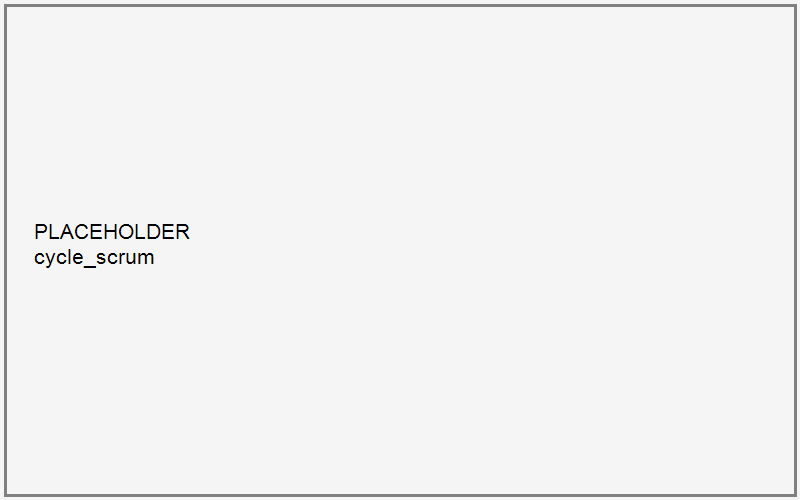
\includegraphics[width=12cm]{image/ChatGPT Image Aug 8, 2026, 07_07_47 PM.png}
    \caption{Cycle de travail Scrum adopté pour la conduite du projet}
    \label{fig:cycle-scrum}
\end{figure}

\subsection*{Organisation de l'équipe Scrum}

La méthodologie Scrum s'appuie sur trois rôles principaux :

\paragraph{Product Owner}\mbox{}\par
Le Product Owner représente les besoins des utilisateurs et définit la vision du produit. Il est chargé de gérer et de prioriser le backlog afin de maximiser la valeur du projet. Ses principales responsabilités sont :
\begin{itemize}
    \item Définir et prioriser les fonctionnalités ;
    \item Planifier les différentes releases ;
    \item Ajuster les priorités en fonction des besoins ;
    \item Valider les fonctionnalités développées.
\end{itemize}

\paragraph{Scrum Master}\mbox{}\par
Le Scrum Master veille au respect des principes Scrum et facilite la collaboration entre les membres de l'équipe. Il accompagne également l'équipe dans la résolution des obstacles pouvant ralentir le développement.

\paragraph{Équipe de développement}\mbox{}\par
L'équipe de développement est responsable de la conception, de l'implémentation et des tests des différentes fonctionnalités du système afin d'atteindre les objectifs fixés pour chaque sprint.

\subsection*{Répartition des rôles}

Dans le cadre de notre projet, les rôles Scrum sont répartis comme suit :
\begin{itemize}
    \item Product Owner : encadrant académique et encadrant professionnel au sein de NextStep IT ;
    \item Scrum Master : Arafet Ben Kilani ;
    \item Équipe de développement : Adel Bettaieb.
\end{itemize}

\subsection*{Planification dans Scrum}

La méthodologie Scrum s'appuie principalement sur trois concepts : le Sprint (période de développement durant laquelle un ensemble de fonctionnalités est réalisé), la Release (version du produit regroupant un ou plusieurs sprints validés), et le Weekly Scrum : compte tenu de l'organisation mono-développeur du projet, la réunion de suivi n'est pas tenue quotidiennement mais de façon hebdomadaire, permettant de suivre l'avancement des travaux, d'identifier les difficultés rencontrées et de coordonner les tâches à réaliser pour la semaine suivante.

\section{Conclusion}

Dans ce chapitre, nous avons présenté l'organisme d'accueil ainsi que le contexte général du projet. Nous avons ensuite exposé la problématique, étudié les solutions existantes et comparé plusieurs méthodologies de développement afin de justifier le choix de Scrum. Le chapitre suivant est consacré à l'analyse et la spécification des besoins de la plateforme.
